
\documentclass[11pt]{amsart}
\usepackage[english]{babel}
\usepackage[margin=1.6in]{geometry}
\usepackage{amsmath}
\usepackage{amsfonts}
\usepackage{amssymb}
%\usepackage{showlabels}
\usepackage{amsthm}

\usepackage[english]{babel}
\usepackage{yfonts}
\usepackage[T1]{fontenc}
\usepackage[utf8x]{inputenc}
\usepackage{enumerate}
\usepackage{enumitem}
\usepackage{verbatim}
\usepackage{graphicx}
\usepackage{verbatim}
\usepackage{faktor}
\usepackage{xcolor}
\usepackage{xfrac}
\usepackage{tikz,tikz-cd}
\usepackage[all]{xy}
\usepackage{hyperref}
\usepackage[normalem]{ulem}

\usepackage{calrsfs}
\DeclareMathAlphabet{\pazocal}{OMS}{zplm}{m}{n}

\newcommand{\M}[4]{\overline{\pazocal M}_{#1,#2}(#3,#4)}
\newcommand{\PP}{\mathbb P}
\renewcommand{\k}{\mathbf k}
\newcommand{\m}{\mathfrak m}
\newcommand{\tR}{\widetilde{R}}
\newcommand{\tm}{\widetilde{\mathfrak m}}
\newcommand{\OO}{\mathcal O}
\renewcommand{\to}{\rightarrow}
\newcommand{\pr}{\rm{pr}}
\newcommand{\Aaff}{\mathbb A}
\newcommand{\N}{\mathbb N}
\newcommand{\oM}{\overline{\pazocal M}}
\newcommand{\tM}{\widetilde{\pazocal M}}
\newcommand{\R}{\operatorname{R}}
\newcommand{\Gm}{\mathbb{G}_{\rm{m}}}
\newcommand{\Ga}{\mathbb{G}_{\rm{a}}}
\newcommand{\vir}[1]{[#1]^{\rm{vir}}}
\newcommand{\virloc}[1]{[#1]^{\rm{vir}}_{\rm{loc}}}
\newcommand{\dvr}{\Delta}

\newcommand{\bq}{\begin{equation}}
\newcommand{\eq}{\end{equation}}
\newcommand{\ba}{\begin{aligned}}
\newcommand{\ea}{\end{aligned}}
\newcommand{\be}{\begin{enumerate}}
\newcommand{\ee}{\end{enumerate}}
\newcommand{\bsm}{\left(\begin{smallmatrix}}
\newcommand{\esm}{\end{smallmatrix}\right)}                   
\newcommand{\bpm}{\begin{pmatrix}}
\newcommand{\epm}{\end{pmatrix}}
\newcommand{\barr}{\begin{displaymath}\begin{array}{cccc}}
\newcommand{\earr}{\end{array}\end{displaymath}}
\newcommand{\barrl}{\begin{displaymath}\begin{array}{lcl}}
\newcommand{\earrl}{\end{array}\end{displaymath}}
\newcommand{\barl}{\begin{displaymath}\begin{array}{l}}
\newcommand{\earl}{\end{array}\end{displaymath}}
\newcommand{\bxym}{ \begin{displaymath}\xymatrix }
\newcommand{\exym}{\end{displaymath}}
\newcommand{\bcd}{\begin{center}\begin{tikzcd}}
\newcommand{\ecd}{\end{tikzcd}\end{center}}

\newcommand{\tr}{{\rm tr}}
\newcommand{\Isom}{\text{Isom}}
\newcommand{\Spec}{\underline{\operatorname{Spec}}}
\newcommand{\Proj}{\operatorname{Proj}}
\newcommand{\Pic}{\operatorname{Pic}}
\newcommand{\Hom}{\operatorname{Hom}}
\newcommand{\hhom}{\mathcal{H}\!om}
\newcommand{\Aut}{\operatorname{Aut}}
\newcommand{\lev}{\operatorname{lev}}
\newcommand{\id}{{\rm id}}

\theoremstyle{plain}
\newtheorem{thm}{Theorem}[section]
\newtheorem{conj}{Conjecture}
\newtheorem{lem}[thm]{Lemma}
\newtheorem{prop}[thm]{Proposition}
\newtheorem{defprop}[thm]{Definition-Proposition}
\newtheorem{cor}[thm]{Corollary}
\newtheorem*{teo*}{Theorem}
\newtheorem*{matteo*}{Main Theorem}
\newtheorem{ipotesi}{ipotesi}
\newtheorem*{nota}{Nota}
\newtheorem{claim}{Claim}
\newtheorem{question}[thm]{Question}

\theoremstyle{definition}
\newtheorem{example}[thm]{Example}
\newtheorem{ex}[thm]{Example}
\newtheorem{dfn}[thm]{Definition}
\newtheorem{remark}[thm]{Remark}
\newtheorem{com}[thm]{Comment}
\newtheorem{num}{Number}
\newtheorem*{sketch}{Sketch}
\newtheorem{rem}[thm]{Remark}


\newcommand{\todo}[1]{\vspace{5mm}\par \noindent
\framebox{\begin{minipage}[c]{0.95 \textwidth} \tt #1\end{minipage}} \vspace{5mm} \par}

\def\ti{-\allowhyphens}
\newcommand{\thismonth}{\ifcase\month % case 0 --- impossible!
  \or January\or February\or March\or April\or May\or June%
  \or July\or August\or September\or October\or November%
  \or December\fi}
\newcommand{\thismonthyear}{{\thismonth} {\number\year}}
\newcommand{\thisdaymonthyear}{{\number\day} {\thismonth} {\number\year}}

\title{Modular compactifications of $\pazocal{M}_{2,n}$}
\author{Luca Battistella}
\date{\today}

\setcounter{tocdepth}{1}
\begin{document}

\begin{abstract}


\end{abstract}

\maketitle
\tableofcontents

\section{Gorenstein curve singularities of genus two}
In this and the next sections we work over an algebraically closed field of characteristic different from $2,3,5$.

We follow Smyth's procedure; let $(R,\m)$ denote the completion of the local ring of the curve at the singularity, with normalisation:
\[(\tR,\tm)\simeq\left(\k[[t_1]]\oplus\ldots\oplus\k[[t_m]],\langle t_1,\ldots,t_m\rangle\right).\]
Hence $m$ is the number of branches. Recall that:
\[g=\delta-m+1,\]
so $\delta=m+1$ in our case. It is an observation of Smyth that $\tR/R$ is graded by:
\[ (\tR/R)_i:=\tm^i/(\tm^i\cap R)+\tm^{i+1};\]
furthermore he notices that:
\begin{enumerate}
\item $m+1=\delta(p)=\sum_{i\geq 0}\dim_\k(\tR/R)_i;$
\item $2=g=\sum_{i\geq 1}\dim_\k(\tR/R)_i;$
\item if $(\tR/R)_i=(\tR/R)_j=0$ then $(\tR/R)_{i+j}=0$.
\end{enumerate}
The following facts will also turn out to be useful:
\begin{enumerate}[resume]
 \item $\sum_{i\geq k}(\tR/R)_i$ is a grading of $\tm^k/(\tm^k\cap R)$;
 \item the following exact sequence holds:
 \[ 0\to \frac{\tm^k\cap R}{\tm^{k+1}\cap R}\to \frac{\tm^k}{\tm^{k+1}}\to \left(\tR/R\right)_k\to 0\]
\end{enumerate}
We proceed by increasing number of branches.
\begin{enumerate}[label={\textbf{Case $m=$}\arabic*:}]

 \item Notice that in the unibranch case $\dim_\k(\tR/R)_1\leq 1$, hence equality must hold (by observation (3) above). We are thus left with two cases:
 \begin{itemize}[leftmargin=0pt]
  \item either $\dim_\k(\tR/R)_2=1$ and $\dim_\k(\tR/R)_i=0$ for all $i\geq 3$: in this case $\tm^3\subseteq\m$ by observation (4). In facts by (5) we see that \[\tm^3=\m\], hence $R\simeq\k[[t^3,t^4,t^5]],$ a non-Gorenstein singularity.
  
  \item or $\dim_\k(\tR/R)_3=1$ and $\dim_\k(\tR/R)_i=0$ for $i=2$ and for all $i\geq 4$: in this case $\tm^4\subseteq\m$ by observation (4). On the other hand from $\dim_\k(\tm^2\cap R/\tm^3\cap R)=1$ we deduce that there is a generator of degree $2$, and from $\dim_\k(\tm^3\cap R/\tm^4\cap R)=0$ there is none of degree $3$; so we see that \[\m/\m^2=\langle t^2,t^5\rangle,\] i.e. $R\simeq\k[[x,y]]/(x^5-y^2)$.
 \end{itemize}

 
 \item This time we have three cases:
 \begin{itemize}[leftmargin=0pt]
  \item $\dim_\k(\tR/R)_1=2$ and $\dim_\k(\tR/R)_i=0$ for all $i\geq 2$: in this case $\tm^2\subseteq\m$ by observation (4); in facts they are equal. Then \[\m/\m^2=\langle t_1^2,t_1^3,t_2^2,t_2^3\rangle\] is the transversal union of two cusps in $\Aaff^4_\k$.
  \item $\dim_\k(\tR/R)_1=\dim_\k(\tR/R)_2=1$ and $\dim_\k(\tR/R)_i=0$ for all $i\geq 3$: in this case $\tm^3\subseteq\m$ by observation (4).
 There is a generator which we may assume is of the form: 
 \[f_1=t_1+at^n_2\in\m\;\;\text{for}\;\; n=1,2;\] on the other hand $\tm^2\cap R$ is spanned by $f_1^2$. Now, if $a=0$, does not matter if $n=1$ or $2$ and we have \[\m/\m^2=\langle t_1,t_2^3,t_2^4,t_2^5\rangle\] is the union of the non-Gorenstein unibranch singularity with a transversal axis. Otherwise we have two cases, in both we can assume wlog $a=1$. 
 \begin{description}[leftmargin=0pt]
 \item[$n=1$] then $\tm^4\subseteq\m^2$, hence \[\m/\m^2=\langle f_1,t_2^3\rangle\] and $R\simeq k[[x,y]]/y(x^3-y)$, so we have the union two smooth branches intersecting along a length $3$ sub-scheme.
 \item[$n=2$] then in $\m$ we have $t_1^2=f_1^2-t_2^4$ since $t_2^4\in\tm^3\subseteq\m;$ however this latter element in not in $\m^2$, so
 \[\m/\m^2=\langle f_1=t_1+t_2^2,t_1^2,t_2^3\rangle.\]
 The singularity we have in this case is a union of a cusp and a smooth branch (a parabola) in the 3-space with intersection of length $2$.
 \end{description}
  \item $\dim_\k(\tR/R)_1=\dim_\k(\tR/R)_3=1$ and $\dim_\k(\tR/R)_i=0$ for $i=2$ and for all $i\geq 4$: in this case $\tm^4\subseteq\m$ by observation (4). Again there is a generator of the form \[f_1=t_1+at_2^n\in\m\;\;\text{for}\;\;n=1,2,3\] but this time there is also a "quadratic generator" $f_2$ which is independent from $f_1^2$, so it has to be of the form \[f_2=bt_1^m+t_2^2\;\;\text{ for} \;\;m=2,3.\] On the other hand $f_1^3$ and $f_1f_2$ are linearly dependent modulo $\tm^4\subset\m$.
\begin{description}[leftmargin=0pt]
\item[$n=1, m=2$]In this case $f_1^3$ and $f_2f_1$ are already in $\tm^3\cup R/\tm^4$ so they need to be linearly dependent; a computation shows then that $a=0$, (otherwise we would get $f_1^2$ and $f_2$ proportional) i.e. $f_1=t_1$ and we may as well assume that $f_2=t_2^2$. Finally 
  \[\m/\m^2=\langle t_1,t_2^2,t_2^5\rangle\] 
  is the union of the Gorenstein unibranch singularity with a transversal axis. 
  \item[$n=1, m=3$] We can assume $a,b\neq 0$ otherwise we fall back in the above case; but then we see that this case does not occur because the linear dependence modulo $\tm^4$ can't be satiisfies if $a\neq 0$.
  \item[$n=2, m=2$] We can assume $a=1$ otherwise we are in the previous case; imposing linear dependence of $f_1^3,f_1f_2$ up to $\tm^4$ we find $b\neq 0$, so we may assume it is one as well and we have  \[\m/\m^2=\langle t_1+t^2,t_1^2+t_2^2,t_2^5\rangle.\]
  A change of variables show that in fact this singularity is isomorphic to the union of the ramphoidal cusp with a transversal axis. 
  \item[$n=2, m=3$] Once again we can assume $a,b\neq 0$ otherwise we are back to the $n=1,m=2$ case. Then we have that $f_1f_2$ is zero mod $\tm^4$ and $\tm^3\cup R/\tm^4$ is generated by $f_1^3.$ Once again we have 
  \[\m/\m^2=\langle f_1,f_2,t_2^5\rangle\]
  and also the singularity is isomorphic to the one above.
  \item[$n=3, m=2$] We can assume that $a=1$ for the formentioned reason and it easy to see that we can always reduce to the case where the second generator has $b=0;$ the we compute the generators to be:  \[\m/\m^2=\langle f_1=t_1+t_2^3,f_2=t_2^2,\rangle\]
  and thus we get a planar singularity with local equation $x(y^2-x^3),$ i.e. the union of a line and a cusp in the plane intersecting in a length $2$ sub-scheme.
  \item[$n=3, m=3$] The same type of arguments we have been using so far shows that in this case we get again the planar singularity $x(y^2-x^3).$
  \end{description}
 \end{itemize}
\end{enumerate}

\begin{remark}
It seems that the genus $2$ case is significantly more difficult that the genus $1$ due to the fact that in this case we need to consider non homogeneous generators. It does seem hopeless to perform the classification for an arbitrary number of branches.
 However, we see that each 2-branches genus $2$ singularity is obtained by gluing two singularities $R_1$ and $R_2$ with $g(R_i)\leq 2$ along a closed sub-scheme of length $\leq 3.$ 
 This is clear if we look at the factorisation of the normalisation $R\hookrightarrow \widetilde{R}=k[[t_1]]\oplus k[[t_2]]$ 
 through $R\hookrightarrow R_1\oplus \R_2\hookrightarrow \widetilde{R},$ where 
 the first partial normalisation correspond to separate the branches. Algebraically this can be achieved considering the $k$ subvector space $K^{\rm{br}}$ of $\widetilde{R}/R$ generated by those conditions involving only one branch at the time an then taking the Kernel of $\widetilde{R}\to K^{\rm{br}}.$
\end{remark}

\begin{prop}
 There is a unique Gorenstein singularity of genus two that is unibranch; for every number of branches $m\geq 2$, there are two.
\end{prop}
\begin{proof}
 I discuss the case $m\geq 3$. Recall that $\delta=m+g-1=m+1=\dim_\k(\tR/R)$. The latter is filtered by $(\tR/R)_k:=\frac{\tm^k}{(\tm^k\cap R)+\tm^{k+1}}$, which fit in the exact sequence
 \[0\to A_k:=\frac{\tm^k\cap R}{\tm^{k+1}\cap R}\to \frac{\tm^k}{\tm^{k+1}}\to(\tR/R)_k\to 0.\]
 All of them are $R/\m=\k$-modules. The middle term has dimension $m$ for every $k$, and $A_0=\k$, so $\dim_{\k}(\tR/R)_0=m-1$. On the other hand \[(\tR/R)_i=0,(\tR/R)_j=0\Rightarrow(\tR/R)_{i+j}=0,\]
 so we only have three possibilities as for what the dimension of $(\tR/R)_i,i=1,2,3,$ can be. Let $I_p$ denote the conductor ideal.
 
 \textbf{Case I}: $(2,0,0)$. In this case $\tm^2\subseteq I_p$, so (by the Gorenstein assumption) $m+1=\delta=\dim_\k(R/I_p)\leq \dim_\k(R/\tm^2)=\dim_\k A_0+\dim_k A_1=m-1$, contradiction.
 
 \textbf{Case II}: $(1,1,0)$. In this case $\tm^3\subseteq I_p$. We are going to write down the $m-1$ generators of $A_1$ ($\operatorname{mod} \tm^3$). The first one, call it, $x_1$, has a non-trivial linear term in at least one of the variables, wlog $t_1$. We can therefore change coordinates in $t_1$ and make it into the form:
 $x_1=t_1\oplus p_{1,2}(t_2)\oplus\ldots\oplus p_{1,m}(t_m) \mod\tm^3.$ Now we can use $x_1$ and $x_1^2$ to make the second generator start with a $0$. It will still have a linear term independent of $t_1$, say non-trivial in $t_2$. Now by changing coordinates in the latter, we can write $x_2=0\oplus t_2\oplus\ldots\oplus p_{1,m}(t_m) \mod\tm^3.$ Also notice that, by taking a linear combination with $x_2$ and $x_2^2$, we may assume that $x_1=t_1\oplus0\oplus p_{1,3}(t_3)\oplus\ldots\oplus p_{1,m}(t_m)\mod\tm^3$. Therefore, by Gaussian elimination and coordinate change, we may write
 \begin{align*}
  x_1= & t_1\oplus0\oplus\ldots\oplus\alpha_{1,m}t_m+\beta_{1,m}t_m^2\\
  x_2= & 0\oplus t_2\oplus\ldots\oplus\alpha_{2,m}t_m+\beta_{2,m}t_m^2\\
  &\ldots\\
  x_{m-1}= & 0\oplus\ldots\oplus t_{m-1}\oplus\alpha_{m-1,m}t_m+\beta_{m-1,m}t_m^2\\
 \end{align*}
 ($\operatorname{mod}\tm^3$). We must have $R/I_p=\langle 1,x_1,\ldots,x_{m-1},y\rangle$ by the Gorenstein condition (if $x_i\in I_p$, then $t_i\in R$, and it is then easy to see that the singularity is decomposable). Now $x_i^2\in I_p$ for all but at most one $i$, say $i=1$. Then $t_i^2\in R$ for $i=2,\ldots,m-1$. If $\alpha_{i,m}\neq 0$ for some $i$ in this range, then $t_m^2\in R$ as well, so $t_{m-1}^2=x_{m-1}^2-O(t_m^2)\in R$, contradicting $\dim_\k(\tR/R)_2=1$. Therefore $\alpha_{i,m}=0$ for $i\in\{2,\ldots,m-1\}$. If $\alpha_{1,m}=0$, then we need a further generator of $\m/\m^2$, namely $z=0\oplus\ldots\oplus t_m^3$. In this case, though, both $x_{m-1}^2$ and $z$ belong to $I_p$, so $\dim_k(R/I_p)=m$, and the singularity cannot be Gorenstein. Finally, if $\alpha_{1,m}\neq 0$, by changing coordinates in $t_m$ and scaling each generator, we find:
 \begin{align}\label{coordII}
 \begin{split}
  x_1= & t_1\oplus0\oplus\ldots\oplus t_m\\
  x_2= & 0\oplus t_2\oplus\ldots\oplus t_m^2\\
  &\ldots\\
  x_{m-1}= & 0\oplus\ldots\oplus t_{m-1}\oplus t_m^2.
 \end{split}
 \end{align}
 We may check that $R/I_p=\langle 1,x_1,\ldots,x_{m-1},x_1^2\rangle$ and $\tR/R$ is of type $(1,1,0)$. In the case $m=2$, we need an extra generator $y=t_2^3$. Equations are given by
 \begin{itemize}
  \item $y(y-x_1^3)$ if $m=2$ ($A_5$-singularity);
  \item $x_1x_2(x_2-x_1^2)$ if $m=3$ ($D_6$-singularity);
  \item $\langle x_3(x_1^2-x_2),x_i(x_j-x_k)\rangle_{1\leq i<j<k\leq m-1 \text{ or }1<j<k<i\leq m-1}$ if $m\geq 4$.
 \end{itemize}

 
 \textbf{Case III}: $(1,0,1)$. We have $\tm^4\subseteq I_p$. By an argument similar to the above, we write generators for $A_1$ as $x_i=\ldots\oplus t_i\oplus\ldots \oplus\alpha_{i,m}t_m+\beta_{i,m}t_m^2+\gamma_{i,m}t_m^3$, for $i=1,\ldots,m-1$. Then $R/I_p=\langle 1,x_1,\ldots,x_{m-1},y\rangle$. For all but at most one $i$, say $i=1$, $x_i^2\in I_p$. On the other hand $t_m^3\notin R$, because otherwise $t_i^3=x_i^3-\alpha_{i,m}^3t_m^3+O(t_m^4)$ belongs to $R$ as well, contradicting $\dim_\k(\tR/R)_3=1$. We deduce that $\alpha_{i,m}=0$ for $i=2,\ldots,m-1$. If $\alpha_{1,m}\neq0$, by changing coordinates in $t_m$, we could write $x_1=t_1\oplus\ldots\oplus t_m$. But $x_1^3\in I_p$ implies $t_m^3\in R$. Therefore $\alpha_{1,m}=0$ and, up to a coordinate change, we may write $x_1=t_1\oplus\ldots\oplus t_m^2$. By $\dim_\k(\tR/R)_2=0$ we find another generator $z=t_m^2+\gamma_zt_m^3$ of $\m/\m^2$. We can use $z$ to remove all the $t_m^2$ pieces from $x_1,\ldots,x_{m-1}$. Finally, we change coordinates in $t_m$ so that $z=t_m^2$, and we scale all the previously found generators so that
 \begin{align}\label{coordIII}
 \begin{split}
  x_1= & t_1\oplus0\oplus\ldots\oplus t_m^3\\
  x_2= & 0\oplus t_2\oplus\ldots\oplus t_m^3\\
  &\ldots\\
  x_{m-1}= & 0\oplus\ldots\oplus t_{m-1}\oplus t_m^3\\
  x_m= & 0\oplus\ldots\oplus t_m^2.
  \end{split}
 \end{align}
 We may check that $R/I_p=\langle 1,x_1,\ldots,x_{m-1},x_m\rangle$ and $\tR/R$ is of type $(1,0,1)$. The case $m=1$ is given by the subalgebra $\k[t^2,t^5]\subseteq\k[t]$. Equations are given by
 \begin{itemize}
  \item $x^5-y^2$ if $m=1$ ($A_4$-singularity or \emph{ramphoid cusp});
  \item $y(y^3-x^2)$ if $m=2$ ($D_5$-singularity);
  \item $\langle x_3(x_1-x_2),x_3^3-x_1x_2\rangle$ if $m=3$;
  \item $\langle x_i(x_j-x_k), x_m(x_i-x_j),x_m^3-x_1x_2\rangle_{i,j,k\in\{1,\ldots,m-1\}\text{ all different}}$ if $m\geq 4$.
 \end{itemize}
\end{proof}

\begin{rem}
 Notice that singularities of type II do appear in the miniversal deformation of singularities of type III, and viceversa. This can be seen for low values of $m$, thanks to a beautiful result of Grothendieck:
 \begin{thm}
  Let $(C,p)$ be a singularity of ADE type. Singularities that appear in the miniversal deformation of $(C,p)$ are all and only those ADE, whose Dynkin diagram can be obtained as a full subgraph of the diagram of $(C,p)$.
 \end{thm}
\end{rem}

\begin{dfn}
 In case II, we shall call the branches parametrised by $t_1$ and $t_m$ \emph{twin}; in case III, the branch parametrised by $t_m$ is called the \emph{singular} branch. We shall refer to them as \emph{special} or \emph{distinguished} branches; all other branches are referred to as \emph{axes}. \emph{Branch} remains a generic name, indicating any of the previous ones.
\end{dfn}


\section{Tangent sheaf and automorphisms}
\begin{prop}
 Describes the tangent sheaf of a genus two singularity in local coordinates.
\end{prop}
\begin{proof}
 Let $\nu\colon\tilde C\to C$ be the normalisation map, and $K(\tilde C)$ the constant sheaf of rational functions on $\tilde C$. A section of $\Omega_{\tilde C}^\vee\otimes K(\tilde C)$ is contained in $\Omega_C^\vee$ if and only if its image under the push-forward map
 \[\nu_*\colon\nu_*\hhom(\Omega_{\tilde C},K(\tilde C))\to \hhom(\Omega_C,K(\tilde C)) \]
 lies in the subspace $\hhom(\Omega_C,\OO_C)$. We may work formally around the singular point in the coordinates given above.
\begin{description}
 \item[$A_4$] In the coordinates $x=t^2,y=t^5$, the section $f(t)\frac{d}{dt}\in\nu_*\Omega_{\tilde C}^\vee\otimes K(\tilde C)$ pushes forward to
 \[\nu_*\left(f(t)\frac{d}{dt}\right)=2tf(t)\frac{d}{dx}+5t^4f(t)\frac{d}{dy},\]
 from which, writing $f(t)=f_0+f_1t+f_2t^2+O(t^3)$, we see that
 \[2tf(t),5t^4f(t)\in\hat\OO_{C,p}\Leftrightarrow f_0=f_2=0.\]
 \item[$A_5$] In the coordinates $x=t_1\oplus t_2,y=t_1^3$, the section $f_1(t_1)\frac{d}{dt_1}\oplus f_2(t_2)\frac{d}{dt_2}$ pushes forward to
 \[\nu_*\left(f_1(t_1)\frac{d}{dt_1}\oplus f_2(t_2)\frac{d}{dt_2}\right)=\left(f_1(t_1)\oplus f_2(t_2)\right)\frac{d}{dx}+3t_1^2f_1(t_1)\frac{d}{dy},\]
 from which, writing $f_i(t_i)=f_{i0}+f_{i1}t_i+f_{i2}t_i^2+O(t_i^3),i=1,2$, we see that
 \[f_1(t_1)\oplus f_2(t_2),3t_1^2f_1(t_1)\in\hat\OO_{C,p} \Leftrightarrow \begin{cases} f_{10}=f_{20}=0,\\ f_{11}=f_{21},\\ f_{12}=f_{22}.\end{cases}\]
 \item[$I\!I_{m\geq 3}$] In the coordinates of \eqref{coordII},
 \[\nu_*\left(\sum_{i=1}^m f_i(t_i)\frac{d}{dt_i}\right)=\left(f_1(t_1)\oplus f_m(t_m)\right)\frac{d}{dx_1}+\sum_{i=2}^m\left(f_i(t_i)\oplus2t_mf_m(t_m)\right)\frac{d}{dx_i},\]
 hence we deduce that
 \[\nu_*\left(\sum_{i=1}^m f_i(t_i)\frac{d}{dt_i}\right)\in\Omega_C^\vee\otimes\hat\OO_{C,p}\Leftrightarrow \begin{cases} f_{i0}=0 & \text{for } i=1,\ldots,m,\\ 2f_{11}=f_{i1}=2f_{m1}, & \text{for } i=2,\ldots,m-1,\\ f_{12}=f_{m2}.\end{cases}\]
  \item[$I\!I\!I_{m\geq 2}$] In the coordinates of \eqref{coordIII},
 \[\nu_*\left(\sum_{i=1}^m f_i(t_i)\frac{d}{dt_i}\right)=\sum_{i=1}^{m-1}\left(f_i(t_i)\oplus3t_m^2f_m(t_m)\right)\frac{d}{dx_i}+2t_mf_m(t_m)\frac{d}{dx_m},\]
 hence we deduce that
 \[\nu_*\left(\sum_{i=1}^m f_i(t_i)\frac{d}{dt_i}\right)\in\Omega_C^\vee\otimes\hat\OO_{C,p}\Leftrightarrow \begin{cases} f_{i0}=0 & \text{for } i=1,\ldots,m,\\ f_{i1}=3f_{m1}, & \text{for } i=1,\ldots,m-1,\\ f_{m2}=0.\end{cases}\]
\end{description}
\end{proof}

Recall Smyth's description of Gorenstein curves of genus one with no automorphisms \cite[Proposition 2.3, Corollary 2.4]{SMY1}.

\begin{dfn}
 Let $(C,p_1,\ldots,p_n)$ be a pointed Gorenstein curve. A connected subcurve $D\subseteq C$ is said to be \emph{nodally attached} if $D\cap\overline{C\setminus D}$ consists of nodes only. Let us call a point \emph{special} if it is either a marking or a node. For a nodal and nodally attached subcurve $D$ with normalisation $\nu\colon \tilde D\to D$, pointed by $\nu^{-1}(\{p_1,\ldots,p_n\}\cap D)\cup (D\cap\overline{C\setminus D})\cup\{q\in D|q\text{ node of } D\}$, we shall say that \emph{DM stability holds} if every rational component has at least three special points, and every elliptic component has at least one. We say that $C$ is \emph{rDM} if DM stability holds for every nodal and nodally attached subcurve of $C$.
\end{dfn}

\begin{cor}
 Let $(C,p_1\ldots,p_n)$ be a pointed Gorenstein curve of arithmetic genus two. The condition $H^0(C,\Omega_C^\vee(-\sum_{i=1}^n p_i))=0$ is equivalent to either of the following:
 \begin{enumerate}[leftmargin=.6cm]
  \item $C$ has an $A_4$ singularity with at least one special point, and is rDM.
  \item $C$ has a singularity of type $I\!I_{m\geq 2}$: at least one of its twin branches contains a special point, each of its axes contains at least one special point, and at least one branch has at least two. Furthermore $C$ is rDM.
  \item $C$ has a singularity of type $I\!I\!I_{m\geq 2}$: each of its axes contains at least one special point, and at least one branch has at least two. Furthermore $C$ is rDM.
  \item $C$ has two elliptic $m$-fold points: each of their branches contains at least one special point, and either they share a branch, or at least one branch of each singular point contains at least two special points. Furthermore $C$ is rDM.
  \item $C$ has one elliptic $m$-fold point: if one of its branches is a genus one curve, then all the other ones contain at least a special point; if two of its branches coincide, then all branches contain at least one special point; otherwise, all branches contain at least one special point, and at least one branch has at least two. Furthermore $C$ is rDM.
  \item $C$ has only nodes and is rDM.
 \end{enumerate}
\end{cor}

\section{Dualising line bundle and semistable tails}
This is the most delicate and combinatorially delicate section of the paper. We classify the nodal subcurves that can be contracted in a one-parameter smoothing in order to obtain a Gorenstein singularity of genus two. The upshot is that the shape of the curve depends on one parameter only, namely the distance of the distinguished (i.e. twin or singular) branches from the core (minimal subcurve of genus two), no matter what the latter is. This is going to play a key role in the proof that our moduli spaces are proper.

\begin{rem}
 Smyth's contraction lemma \cite[Lemma 2.13]{SMY1} carries over essentially unchanged.
\end{rem}
\begin{lem}
 Let $\nu\colon\tilde C\to C$ be the normalisation of a Gorenstein singularity of genus two, with $\nu^{-1}(p)=\{p_1,\ldots,p_m\}$. Then $\nu^*\omega_C=\omega_{\tilde C}(3p_1+2p_2+\ldots+2p_{m-1}+3p_m)$ (case II) or $\nu^*\omega_C=\omega_{\tilde C}(2p_1+\ldots+2p_{m-1}+4p_m)$ (case III).
\end{lem}
\begin{proof}
 Recall the explicit description of the dualising sheaf for curves:
 \[\omega_C(U)=\{\eta\in \Omega_{\tilde C}\otimes K(\nu^{-1}(U)) | \sum_{p_i\in\nu^{-1}(p),p\in U}\operatorname{Res}_{p_i}((\nu^*f)\eta)=0,\ \forall f\in\OO_C(U)\}.\]
 In case II, we know that $\tm^3\subseteq R$, therefore we have poles of third order at most. It is enough to study the possible polar tails. Let \[\eta=c_1\frac{\operatorname{d}t_1}{t_1^3}+b_1\frac{\operatorname{d}t_1}{t_1^2}+a_1\frac{\operatorname{d}t_1}{t_1}\oplus\ldots\oplus c_m\frac{\operatorname{d}t_m}{t_m^3}+b_m\frac{\operatorname{d}t_m}{t_m^2}+a_m\frac{\operatorname{d}t_m}{t_m}.\]
 From looking at $1\cdot\eta$ we deduce $\sum_{i=1}^m a_i=0$; from $x_i\cdot\eta$ we see $b_1+b_m=0$ (if $i=1$), and $b_i+c_m=0$ (if $i=2,\ldots,m-1$); finally from $x_i^2\cdot\eta$ we have $c_1+c_m=0$ (if $i=1$), and $c_i=0$ (if $i=2,\ldots,m-1$). Therefore $\omega_C/\nu_*\omega_{\tilde C}$ is spanned by
 \begin{align*}
  \frac{\operatorname{d}t_1}{t_1}-\frac{\operatorname{d}t_m}{t_m},\ldots,\frac{\operatorname{d}t_{m-1}}{t_{m-1}}-\frac{\operatorname{d}t_m}{t_m},\frac{\operatorname{d}t_1}{t_1^2}-\frac{\operatorname{d}t_m}{t_m^2},\\
  \bar{\eta}=\frac{\operatorname{d}t_1}{t_1^3}+\frac{\operatorname{d}t_2}{t_2^2}+\ldots+\frac{\operatorname{d}t_{m-1}}{t_{m-1}^2}-\frac{\operatorname{d}t_m}{t_m^3}.
 \end{align*}
In particular $\omega_C$ is generated by $\bar{\eta}$ as an $\OO_C$-module. Hence the first claim.

In case III, we know that $\tm^4\subseteq R$, therefore we have poles of fourth order at most. On the other hand $t_i^2\in R$ for all $i$ implies the part of order three is trivial. So let \[\eta=c_1\frac{\operatorname{d}t_1}{t_1^4}+b_1\frac{\operatorname{d}t_1}{t_1^2}+a_1\frac{\operatorname{d}t_1}{t_1}\oplus\ldots\oplus c_m\frac{\operatorname{d}t_m}{t_m^4}+b_m\frac{\operatorname{d}t_m}{t_m^2}+a_m\frac{\operatorname{d}t_m}{t_m}.\]
 From looking at $1\cdot\eta$ we deduce $\sum_{i=1}^m a_i=0$; from $x_i\cdot\eta$ we see $b_i+c_m=0$ for all $i$, and from $x_i^3\cdot\eta$ we have $c_i=0$ for all $i$. (The statement about third order poles can be evinced from $x_i^2\cdot\eta$ or from $z\cdot\eta$ indifferently.) Therefore $\omega_C/\nu_*\omega_{\tilde C}$ is spanned by
 \begin{align*}
  \frac{\operatorname{d}t_1}{t_1}-\frac{\operatorname{d}t_m}{t_m},\ldots,\frac{\operatorname{d}t_{m-1}}{t_{m-1}}-\frac{\operatorname{d}t_m}{t_m},\frac{\operatorname{d}t_m}{t_m^2}\\
  \bar{\eta}=\frac{\operatorname{d}t_1}{t_1^2}+\ldots+\frac{\operatorname{d}t_{m-1}}{t_{m-1}^2}-\frac{\operatorname{d}t_m}{t_m^4}.
 \end{align*}
In particular $\omega_C$ is generated by $\bar{\eta}$ as an $\OO_C$-module. Hence the second claim.
\end{proof}

\begin{cor}
 The dualising sheaf has multi-degree $(1,0,\ldots,0,1)$ (case II) and $(0,\ldots,0,2)$ (case III) respectively.
\end{cor}

\begin{rem}
 $H^0(C,\Omega_C^\vee(-\sum_{i=1}^np_i))=0$ implies the ampleness of $\omega_C(\sum_{i=1}^np_i)$.
\end{rem}

\begin{rem}
 Recall Smyth's \emph{balancing} condition \cite[Definition 2.11]{SMY1}, generalised by the interior of a circle around the core in \cite{RSPW1}.
\end{rem}

\begin{prop}[Semistable tails] Let $(C,p)$ be a Gorenstein singularity of genus two, with pointed normalisation $\bigsqcup_{i=1}^m(\PP^1,p_i)$. Let $\mathcal C\to\dvr$ be a one-parameter smoothing of $C$, and $\phi\colon\mathcal C^{ps}\to\mathcal C$ a birational contraction from a prestable curve. Let $(Z,p_1,\ldots,p_m)$ be $\phi^{-1}(p)$ marked with the intersection points with the rest of $\mathcal C^{ps}_0$.
 \begin{itemize}[leftmargin=.5cm]
  \item Case II: $p_1$ and $p_m$ are either on the same rational tail, attached to a Weierstrass point, or on two different tails, attached to conjugate points. In any case they are equidistant from the core. All other $p_i$ are further away from it.
  \item Case III: $p_m$ is on a tail attached to a Weierstrass point, all other $p_i$ are further away from the core.
 \end{itemize}
\end{prop}
\begin{proof}
 By Smyth's contraction lemma \cite[Lemma 2.13]{SMY1}, a semistable curve of genus two $(Z,p_1,\ldots,p_m)$ is a semistable tail iff there exists a smoothing $\mathcal C^s\to\dvr$ of a compactification obtained by adjoining an $m$-marked tail to $p_1,\ldots,p_m$, and a line bundle $\mathcal L$ on $\mathcal C^s$ of the form $\omega_{\mathcal C^s/\dvr}(D)$, with $D$ an effective divisor supported on $Z$, such that $\mathcal L$ is ample everywhere except on $Z$, where it restricts to the structure sheaf.
 
 We may split $Z$ into a core $K$ (minimal subcurve of genus two) and a number (possibly zero) of rational trees. \emph{We start by analysing the latter ones.} Observe that, by the previous lemma, in case II $p_1$ and $p_m$ are attached to a component that appears with multiplicity $2$ in $D$ (resp. in case III $p_m$ is attached to a component along which $D$ has multiplicity $3$), while all other markings lie on multiplicity $1$ components.
 
 First, we claim that no component can appear with multiplicity $0$ in $D$. Assume that this occurred along one of the rational trees. Call $S$ such a component, $R$ the one that precedes it, and $T_1,\ldots, T_h$ the ones that follow it (when sweeping the tree from the core), and let $d_A$ denote the multiplicity of the divisor $D$ along the component $A$. Then \[\deg(\mathcal L_{|S})= -2+(h+1)+d_R+\sum d_{T_i}=0,\]
 which implies that all the $d_A$ involved are $0$, since $h\geq1$ by semistability. Also, $h=1$, hence we are looking at a bead of a rational chain. Since this consideration propagates, in the long run we will span the whole of $Z$, hence showing that $Z$ is itself a rational chain, which is absurd.
 %In the long run, this implies that $d_K=0$, but this contradicts $\deg(\mathcal L_{|K})=0$, since the left-hand side is a sum of $\deg(\omega_K(-K))$ with other positive terms.
 
 Second, let's study the case $d_S=1$. We stick to the notation above; furthermore, there can be a number of $p_i$, $i\in\{2,\ldots,m-2\}$, lying on $S$, which we think of as extra tails $T_1^\prime,\ldots,T_k^\prime$ attached to $S$, but lying outside the support of $D$. Then
 \[\deg(\mathcal L_{|S})= -2+(h+k+1)-(h+k+1)+d_R+\sum d_{T_i}=0.\]
 Either $d_R=2$, $h=0$ and $k\geq 1$; or $d_R=1$, $h=1$, and $d_{T_1}=1$ (with $k$ arbitrary). In the latter case, though, we may repeat the argument on $T_1$, and we find an infinite chain in $Z$, which can be excluded. More generally, an analogous computation shows that, when balancing a component $A$ of multiplicity $d_A$, all neighbouring components of multiplicity $d_A-1$ can be safely ignored (at the same time, the number of such components is only bounded by the semistability of $Z$ and the quantity of markings).\footnote{define the trend along a rational chain and show it is unaltered by $\alpha-(\alpha-1)$-interactions}
 
 We now prove that $d_R>d_S$ in general. The previous two paragraphs deal with the case $d_S=0,1$; we may therefore assume $d_S>1$ (which in particular implies $0\leq k\leq 2$). We have
 \[\deg(\mathcal L_{|S})= -2+(h+k+1)+d_R-d_S(h+k+1)+\sum d_{T_i}=0.\]
 By proceeding from leaves to root, we can assume that $d_S>d_{T_i},\ i=1,\ldots,h$. We may therefore rewrite
 \[d_R=(d_S-1)(h+k+1)-\sum d_{T_i}+2\geq(d_S-1)(k+1)+2=d_S+1+k(d_S-1)>d_S.\]
 
In fact, we can prove as on \cite[p.893]{SMY1} that $d_R=d_S+1$, unless $d_S=2$ and either $p_1$ or $p_m$ (or both) are attached to $S$ (type II), or $d_S=3$ and $p_m\in S$ (type III). We single out the former case within the following
\begin{dfn}
 A $1$-tree is a rooted rational tree with weighted vertices, such that its leaves are all at the same distance $l$ from the root $\circ$, and the weight of a vertex $v$ is determined by $d_v=l-\operatorname{dist}(v,\circ)+1$. Legs are attached to leaves only, and every leaf has at least a leg.
\end{dfn}
Let us look at a component $S$ with $d_S=2$ and at least one of $p_1$ and $p_m$ attached to it. The balancing equation is
\[\deg(\mathcal L_{|S})= -2-(h+k+1)+d_R+\sum d_{T_i}=0,\]
with $k\in\{1,2\}$. The preceding discussion implies that $d_{T_i}=1$ for all $i=1,\ldots,h$, so $d_R=3+k$. If $k=2$, both $p_1$ and $p_m$ are on $S$ (therefore they are equidistant from the core). In this case $d_R=5$, and it can be shown inductively that the multiplicity of $D$ along a component increases by $3$ for every step we make towards the core. A similar computation shows that the same property holds in case III, when starting from a component $S$ with $d_S=3$ and $p_m$ attached to it. Let us give the following
\begin{dfn}
 A $3$-chain of weight $w$ is a rooted rational chain of length $l$ such that its leaf has weight $w$ and either one or two distinguished legs. The weight of each vertex $v$ is determined by $w+3(l-\operatorname{dist}(v,\circ))$. A $3$-trunk is obtained by adjoining a finite number of $1$-trees of length $l_i$ to a leg adjacent to a bead of weight $l_i+1$ in a $3$-chain.
\end{dfn}

Finally, say $d_S=2$ and only $p_1\in S$. Then $d_R=4$. It can again be shown that the growth rate along the chain that connects $S$ to the core is usually $2$.
\begin{dfn}
 A $2$-chain is a rooted rational chain of length $l$ such that its leaf has weight $2$ and one distinguished leg. The weight of each vertex $v$ is determined by $2+2(l-\operatorname{dist}(v,\circ))$. A $2$-tree is obtained by adjoining a finite number of $1$-trees of length $l_i$ to a leg adjacent to a bead of weight $l_i+1$ in a $2$-chain. The length of a $2$-tree is the length of its $2$-chain.
\end{dfn}
It is important to notice that this trend can break only when two $2$-trees meet; at that point the growth rate becomes $3$. Hence the following
\begin{dfn}
 A $3$-tree of type II is obtained by adjoining two $2$ trees of the same length $l$ to the two legs of a $3$-trunk of weight $4+l$. A $3$-tree of type III is a $3$-trunk with one leg and weight $3$.
\end{dfn}
It should be clear from the preceding discussion that $Z$ contains a number of $1$-trees (bounded by $m$), and either (a) one $3$-tree or (b) two $2$-trees.
%Call $P$ the component preceding $R$, and $S,Q_1,\ldots,Q_h$ those following it. By studying the degree of $\mathcal L_{|P}$ we find $d_P+\sum d_{Q_i}=6+3h$, and $d_{Q_i}\leq 3$. So $d_P$ is determined (to be $6$), unless one of the $d_{Q_i}$ is $2$, say $i=1$; but in this case $p_m\in Q_1$, so again $p_1$ and $p_m$ are equidistant from the core. This can be generalised: the growth rate on a ``special rational tail'' (one containing either $p_1$ or $p_m$) is determined and higher than that along an ``ordinary rational tail'' (which is $+1$), and it may change only if the two ``special rational tails'' meet.

Finally, let us look at the core $K$. Consider it as a one-pointed (case (a)), resp. two-pointed (case (b)) curve of genus two, by ignoring all the attachment points of the $1$-trees, and let $\bar K\in\oM_{2,1}$ (resp. $\oM_{2,2}$) be its stable model. Recall that $\bar K$ is called Weierstrass if the marking is a fixed-point of the hyperelliptic involution $\sigma$ (case (a)), resp. conjugate if the two markings are swapped by $\sigma$ (case (b)). This is well defined by the existence and uniqueness of a $\mathfrak g^1_2$. More generally, $K$ admits a non-degenerate $2:1$ morphism to $\PP^1$ such that $p_1$ is a ramification point (resp. $\{p_1,p_2\}$ is a fiber) if and only if $\bar K$ does.
\begin{enumerate}

 \item $K$ is a smooth genus two curve. In case (a), the balancing equation admits a solution if and only if $K$ is Weierstrass, while case (b) admits a solution if and only if $K$ is conjugate.
 
 \item $K$ contains two nodally attached irreducible subcurves of genus one $E_1$ and $E_2$. It is convenient to solve the balancing equation on one of them first, say $E=E_1$. If all the neighbouring components have multiplicity $d_E-1$, it's fine. If all but one of the neighbouring components have multiplicity $d_E-1$, then the last one is forced to have multiplicity $d_E-1$ as well. The case that all but two neighbouring components have multiplicity $d_E-1$ occurs when either a $2$-tree or a $3$-tree is attached to $E$ at $q$, and let $F$ be the component going towards $E_2$, with $E\cap F=\{r\}$. The case of a $2$-tree forces $d_F=d_E$ by degree reason, but then we are left to solve $q\sim r$ in $\Pic(E)$, which is impossible; on the other hand, the case of a $3$-tree imposes $d_F=d_E+1$ and $2q\sim 2r$ in $\Pic(E)$, which says that $K$ is Weierstrass. The above considerations imply that, if there are two $2$-trees, they must both be connected to the same $E$ in nodes $q_1,q_2$ such that $q_1+q_2\sim 2r$, and $d_F=d_E+1$. Finally, assume that $E_1$ and $E_2$ are connected by a chain of rational curves $R_i$ in $K$. Then it is easy to see that, if there are two $2$-trees and one of them is connected to an $R_i$, the other must be as well. Furthermore, the incoming growth rate at $E_1$ and $E_2$ must be $1$ in both cases. Hence it can be showed that the rational chain $\{R_i\}$ is symmetric, namely: in case (a) the marking is equidistant from $E_1$ and $E_2$, and in case (b) the distance between a marking and its closest (resp. furthest) $E_i$ are the same for the two markings.
 
 PICTURE
 
 \item $\bar K\in\Delta_{irr}$, or $K$ contains only one nodally attached irreducible subcurve of genus one $E$. $E$ contains two distinguished nodes $r_1$ and $r_2$ joined in $K$ by a (possibly empty) rational chain. We see as above that either a $3$-tree is attached to a point $q\in E$ satisfying $2q\sim r_1+r_2$ in $\Pic(E)$, or two $2$-trees are attached to nodes $q_1,q_2\in E$ satisfying $q_1+q_2\sim r_1+r_2$ in $\Pic(E)$, or the rational chain is not empty and the distinguished trees are attached to it. In this case, solve the balancing equation on $E$: let $d=d_E$, $d_1$ and $d_2$ be the multiplicities of the rational components attached to $r_1$ and $r_2$ respectively; then either $d_1=d_2=d-1$, or $d_1=d-1+k$, $d_2=d-1-k$ and $r_1-r_2$ is $k$-torsion in $\Pic(E)$. But, by chasing the balancing equation along the rational chain, we see that, if $d_1\geq d$, this non-decreasive trend propagates, and in fact increases when passing a distinguished bead, so that we should have $d_2>d$, which is absurd. So again the only possibility is to have a rational chain symmetric with respect to the distinguished beads.
 
 PICTURE
 
 \item Finally, the case that the normalisation of $K$ is a union of $\PP^1$. The only really new case is when a distinguished component contains two nodes such that removing them preserves connectedness. \begin{comment}It can be shown that case (a) admits solution as soon as $K$ is not the union of two $\PP^1$ along three nodes. Case (b) admits a solution if and only if either $q_1$ and $q_2$ belong to different components, or they belong to the same component and $K$ is not the union of two $\PP^1$ along three nodes.\end{comment}
 
 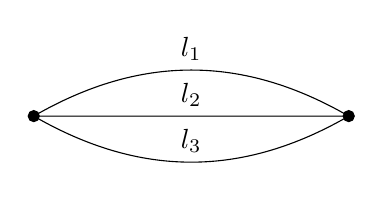
\begin{tikzpicture}
  \draw[fill=black] (0,0) circle(2pt) -- node[above]{$l_2$} (4,0) circle(2pt);
  \draw (0,0) to[out=-30,in=-150] node[above]{$l_3$} (4,0);
  \draw (0,0) to[out=30,in=150] node[above]{$l_1$} (4,0);
 \end{tikzpicture}
Denoting by $l_i$ the length of a rational chain and by $t_i$ the trend along it, balancing reduces to the following system in case (a) and (b).2:\footnote{I am not sure when this admits integral solutions, e.g. not if all $l_i$ are equal}
\[
\begin{pmatrix}
 1 & 1 & 1 \\ l_1+1 & -l_2-1 & 0 \\ l_1+1 & 0 & -l_3-1
\end{pmatrix}
\begin{pmatrix}
 t_1\\ t_2\\ t_3
\end{pmatrix}
=
\begin{pmatrix}
 1 \\ 0 \\ 0
\end{pmatrix}
\]

\end{enumerate}

%Say there are two special tails $T_1$ and $T_m$, intersecting $K$ at $q_1$ and $q_m$, and ordinary tails $T^\prime_1,\ldots,T^\prime_h$, meeting it at $q_1^\prime,\ldots,q_h^\prime$. Then we know from our previous computations that we need $d_K=d_{T_1}+3=d_{T_m}+3$ and $d_K=d_{T_i^\prime}+1$ for all $i$, from which we deduce that $p_1$ and $p_m$ are equidistant from the core even when they are on different rational tails, and all the other $p_i$ are further away; besides this,
%\[\omega_K(-K)(d_KK+d_{T_1}T_1+d_{T_2}T_2+\sum d_{T_i^\prime}T_i^\prime)=\omega_K(-q_1-q_m)\simeq\OO_K\]
%allows us to conclude that $q_1$ and $q_m$ have to be conjugate. In the case that $p_1$ and $p_m$ lie on the same rational tail $T$, the growth rate becomes then $4$, so that $d_K=d_T+4$ and the same computation allows us to conclude that $q$ must be Weierstrass.

\end{proof}

\section{The new moduli functors}
\begin{dfn}
 Let $(C,p_1,\ldots,p_n)$ be a reduced curve, marked by smooth points. For a \sout{nodally attached} subcurve $D\subseteq C$, \textcolor{red}{no matter what the singularities at the intersection with the rest of $C$}, we define the \emph{level} of $D$ to be the number \[ \lev(D)=\lvert D\cap\overline{C\setminus D}\rvert+\lvert\{p_1,\ldots,p_n\}\cap D\rvert.\]
\end{dfn}
\begin{dfn}
 Fix positive integers $m<n$. Let $(C,p_1,\ldots,p_n)$ be a connected, reduced, complete curve of arithmetic genus two, marked by smooth points. We say that $C$ is $m$-stable if:
 \begin{enumerate}
  \item\label{cond:sing} $C$ has only nodes; elliptic $l$-fold points, $l\leq m+1$; type $I\!I_{\leq m+1}$, and type $I\!I\!I_{\leq m}$ genus two singularities as singular points.
  \item\label{cond:lev2} If $Z$ is a connected subcurve of arithmetic genus two, then $\lev(Z)>m$.
  \item\label{cond:lev1} If $E$ is a \sout{nodally attached} subcurve of arithmetic genus one, then $\lev(E)>m+1$.
  \item\label{cond:aut} $H^0(C,\Omega_C^\vee(-\sum_{i=1}^n p_i))=0$.
  \item\label{cond:p1} If $C$ contains a singularity of genus two, $p_1$ is connected (through a rational chain) to one of the distinguished branches.
 \end{enumerate}
\end{dfn}

\begin{rem}
 The definition is not $\mathfrak{S}_n$-symmetric. In the contraction arguments below, we use the asymmetry to write down the dualising line bundle of a genus two (sub)curve $Z$ as $\omega_Z\simeq\OO_Z(q_1+\bar q_1)$, where $q_1$ is the point on $Z$ which is closest to $p_1$. Compare this with the genus one situation, where the dualising line bundle of a Gorenstein curve is trivial.
\end{rem}
\begin{rem}\label{rmk:lev1solev2}
 If there is a subcurve of genus one, condition \eqref{cond:lev1} and condition \eqref{cond:aut} jointly imply condition \eqref{cond:lev2}. Indeed, $\lev(Z)\geq\lev(E)-1$, and the only cases in which the level drops by one are: when $Z=(E,p_1,\ldots,p_{l-2},q_1,q_2)\sqcup_{\{q_1,q_2\}}(\PP^1,q_1,q_2,p_{l-1})$; and when $Z=(E,p_1,\ldots,p_{l-1},q)\sqcup_q(E^\prime,q)$, where $(E^\prime,q)$ is a one-pointed curve of genus one.
\end{rem}


\begin{lem}[boundedness]
 
\end{lem}

\begin{lem}[deformation openness]
 
\end{lem}
\begin{proof}
 Being Gorenstein is an open condition, as much as having connected fibers of arithmetic genus two. This bounds the genus of the singularities that may occur. The case $m=1$ deserves special attention. In this case, that condition \eqref{cond:sing} is open follows from acknowledging that $I\!I_2=A_5$, $I\!I\!I_1=A_4$, while tacnode, cusp, and node are $A_3$, $A_2$, and $A_1$ respectively, and from a beautiful result of Grothendieck concerning the deformation theory of ADE singularities \cite{Arnold,Demazure}. The case $m\geq 2$ simply follows from upper semicontinuity of embedded dimension and the fact that we have exhausted all possible Gorenstein singularities of genus $\leq 2$, and embedding dimension $\leq m+1$.
 
 Condition \eqref{cond:aut} translates to: the locus where the automorphism group is unramified is open in the base.
 
 The other conditions are topological, hence constructible. With Noetherian assumptions, it is enough to check their openness over a dvr scheme. Assume that the geometric generic fiber $C_{\bar\eta}$ contains two genus one subcurve $E_{1,\bar\eta}$ and $E_{2,\bar\eta}$; their closures $E_1$ and $E_2$ in $\mathcal C$ are then flat families of genus one curves over $\dvr$. If $E_{1,\bar\eta}$ and $E_{2,\bar\eta}$ are disconnected, then so are $E_1$ and $E_2$, by local constancy of the number of connected components of fibers of a flat proper morphism with geometrically normal fibers. If $E_{1,\bar\eta}$ and $E_{2,\bar\eta}$ are joined by a (disconnecting) node $q_{\bar\eta}$, then so are $E_{1,0}$ and $E_{2,0}$; indeed, the unique limit of $q_{\bar\eta}$ must be a singular point of the projection, but cannot be any worse than a node by local constancy of the arithmetic genus. Finally, if $E_{1,\bar\eta}$ and $E_{2,\bar\eta}$ share a branch, then so do $E_{1,0}$ and $E_{2,0}$; on the other hand, if $E_{i,\bar\eta}$ has more than one branch, then so does $E_i$. Similarly, if $C_{\bar\eta}$ contains only one subcurve of genus one, with two nodes joined by a rational chain, so does $C_0$. The upshot of this discussion is that
 \[\lvert E_{i,\bar\eta}\cap\overline{C_{\bar\eta}\setminus E_{i,\bar\eta}}\rvert=\lvert E_{i,0}\cap\overline{C_{0}\setminus E_{i,0}}\rvert.\]
 The number of markings on $E_i$ is also constant. Hence we can deduce condition \eqref{cond:lev1} for $C_{\bar\eta}$ from the same condition on $C_0$. Condition \eqref{cond:lev2} follows as in Remark \ref{rmk:lev1solev2}. Condition \eqref{cond:lev2} can be proved analogously when there is no subcurve of genus one.
 
 Finally, suppose that $C_{\bar\eta}$ has a genus two singularity, then so does $C_0$. The (union of the) distinguished branch(es) $E_{\bar\eta}$ of $C_{\bar\eta}$ is a genus one singularity, and so is its limit $E_0$ in $C_0$. It has to contain the distinguished branch(es) of $C_0$, because any subcurve contained in the union of the axes of $C_0$ has genus zero; therefore, by assumption, $E_0$ contains $p_{1,0}$. Then also $E_{\bar\eta}$ contains $p_{1,\bar\eta}$.
\end{proof}



\bibliographystyle{alpha}
\bibliography{genus_two}
\newpage

\noindent Luca Battistella\\
Max Planck Institute for Mathematics - Bonn \\
\texttt{battistella@mpim-bonn.mpg.de}\\


\end{document}

